% Options for packages loaded elsewhere
\PassOptionsToPackage{unicode}{hyperref}
\PassOptionsToPackage{hyphens}{url}
\PassOptionsToPackage{dvipsnames,svgnames,x11names}{xcolor}
%
\documentclass[
  letterpaper,
  DIV=11,
  numbers=noendperiod]{scrartcl}

\usepackage{amsmath,amssymb}
\usepackage{iftex}
\ifPDFTeX
  \usepackage[T1]{fontenc}
  \usepackage[utf8]{inputenc}
  \usepackage{textcomp} % provide euro and other symbols
\else % if luatex or xetex
  \usepackage{unicode-math}
  \defaultfontfeatures{Scale=MatchLowercase}
  \defaultfontfeatures[\rmfamily]{Ligatures=TeX,Scale=1}
\fi
\usepackage{lmodern}
\ifPDFTeX\else  
    % xetex/luatex font selection
\fi
% Use upquote if available, for straight quotes in verbatim environments
\IfFileExists{upquote.sty}{\usepackage{upquote}}{}
\IfFileExists{microtype.sty}{% use microtype if available
  \usepackage[]{microtype}
  \UseMicrotypeSet[protrusion]{basicmath} % disable protrusion for tt fonts
}{}
\makeatletter
\@ifundefined{KOMAClassName}{% if non-KOMA class
  \IfFileExists{parskip.sty}{%
    \usepackage{parskip}
  }{% else
    \setlength{\parindent}{0pt}
    \setlength{\parskip}{6pt plus 2pt minus 1pt}}
}{% if KOMA class
  \KOMAoptions{parskip=half}}
\makeatother
\usepackage{xcolor}
\setlength{\emergencystretch}{3em} % prevent overfull lines
\setcounter{secnumdepth}{-\maxdimen} % remove section numbering
% Make \paragraph and \subparagraph free-standing
\makeatletter
\ifx\paragraph\undefined\else
  \let\oldparagraph\paragraph
  \renewcommand{\paragraph}{
    \@ifstar
      \xxxParagraphStar
      \xxxParagraphNoStar
  }
  \newcommand{\xxxParagraphStar}[1]{\oldparagraph*{#1}\mbox{}}
  \newcommand{\xxxParagraphNoStar}[1]{\oldparagraph{#1}\mbox{}}
\fi
\ifx\subparagraph\undefined\else
  \let\oldsubparagraph\subparagraph
  \renewcommand{\subparagraph}{
    \@ifstar
      \xxxSubParagraphStar
      \xxxSubParagraphNoStar
  }
  \newcommand{\xxxSubParagraphStar}[1]{\oldsubparagraph*{#1}\mbox{}}
  \newcommand{\xxxSubParagraphNoStar}[1]{\oldsubparagraph{#1}\mbox{}}
\fi
\makeatother


\providecommand{\tightlist}{%
  \setlength{\itemsep}{0pt}\setlength{\parskip}{0pt}}\usepackage{longtable,booktabs,array}
\usepackage{calc} % for calculating minipage widths
% Correct order of tables after \paragraph or \subparagraph
\usepackage{etoolbox}
\makeatletter
\patchcmd\longtable{\par}{\if@noskipsec\mbox{}\fi\par}{}{}
\makeatother
% Allow footnotes in longtable head/foot
\IfFileExists{footnotehyper.sty}{\usepackage{footnotehyper}}{\usepackage{footnote}}
\makesavenoteenv{longtable}
\usepackage{graphicx}
\makeatletter
\def\maxwidth{\ifdim\Gin@nat@width>\linewidth\linewidth\else\Gin@nat@width\fi}
\def\maxheight{\ifdim\Gin@nat@height>\textheight\textheight\else\Gin@nat@height\fi}
\makeatother
% Scale images if necessary, so that they will not overflow the page
% margins by default, and it is still possible to overwrite the defaults
% using explicit options in \includegraphics[width, height, ...]{}
\setkeys{Gin}{width=\maxwidth,height=\maxheight,keepaspectratio}
% Set default figure placement to htbp
\makeatletter
\def\fps@figure{htbp}
\makeatother

\KOMAoption{captions}{tableheading}
\makeatletter
\@ifpackageloaded{caption}{}{\usepackage{caption}}
\AtBeginDocument{%
\ifdefined\contentsname
  \renewcommand*\contentsname{Table of contents}
\else
  \newcommand\contentsname{Table of contents}
\fi
\ifdefined\listfigurename
  \renewcommand*\listfigurename{List of Figures}
\else
  \newcommand\listfigurename{List of Figures}
\fi
\ifdefined\listtablename
  \renewcommand*\listtablename{List of Tables}
\else
  \newcommand\listtablename{List of Tables}
\fi
\ifdefined\figurename
  \renewcommand*\figurename{Figure}
\else
  \newcommand\figurename{Figure}
\fi
\ifdefined\tablename
  \renewcommand*\tablename{Table}
\else
  \newcommand\tablename{Table}
\fi
}
\@ifpackageloaded{float}{}{\usepackage{float}}
\floatstyle{ruled}
\@ifundefined{c@chapter}{\newfloat{codelisting}{h}{lop}}{\newfloat{codelisting}{h}{lop}[chapter]}
\floatname{codelisting}{Listing}
\newcommand*\listoflistings{\listof{codelisting}{List of Listings}}
\makeatother
\makeatletter
\makeatother
\makeatletter
\@ifpackageloaded{caption}{}{\usepackage{caption}}
\@ifpackageloaded{subcaption}{}{\usepackage{subcaption}}
\makeatother

\ifLuaTeX
  \usepackage{selnolig}  % disable illegal ligatures
\fi
\usepackage{bookmark}

\IfFileExists{xurl.sty}{\usepackage{xurl}}{} % add URL line breaks if available
\urlstyle{same} % disable monospaced font for URLs
\hypersetup{
  pdftitle={Discrete-Continuous Dynamic Choice Models:},
  pdfauthor={Christophe Bruneel-Zupanc},
  colorlinks=true,
  linkcolor={blue},
  filecolor={Maroon},
  citecolor={Blue},
  urlcolor={Blue},
  pdfcreator={LaTeX via pandoc}}


\title{Discrete-Continuous Dynamic Choice Models:}
\usepackage{etoolbox}
\makeatletter
\providecommand{\subtitle}[1]{% add subtitle to \maketitle
  \apptocmd{\@title}{\par {\large #1 \par}}{}{}
}
\makeatother
\subtitle{Identification and Conditional Choice Probability Estimation}
\author{Christophe Bruneel-Zupanc}
\date{2024-10-29}

\begin{document}
\maketitle


\subsection{Contribution}\label{contribution}

\textbf{Framework:} Simultaneous discrete-continuous choice

\begin{itemize}
\tightlist
\item
  Core identification problem: only observe continuous choice for the
  chosen discrete alternative
\end{itemize}

\textbf{Identification:} Constructive proof of nonparametric
identification

\begin{itemize}
\tightlist
\item
  Instrument: \emph{relevant} for discrete choice, \emph{excluded} from
  continuous choice
\end{itemize}

\textbf{Estimation:} Two-step estimation

\begin{itemize}
\tightlist
\item
  \begin{enumerate}
  \def\labelenumi{\arabic{enumi})}
  \tightlist
  \item
    read CCC and CCP from data\\
  \end{enumerate}
\item
  \begin{enumerate}
  \def\labelenumi{\arabic{enumi})}
  \setcounter{enumi}{1}
  \tightlist
  \item
    structrual estimation to recover parameters
  \end{enumerate}
\end{itemize}

\subsection{Plan}\label{plan}

\begin{itemize}
\tightlist
\item
  \textbf{Framework}: Static
\item
  \textbf{Identification}: Static
\item
  \textbf{Framework}: Dynamic
\item
  \textbf{Identification}: Dynamic
\item
  \textbf{Estimation}
\end{itemize}

\subsection{Framework: Static}\label{framework-static}

\textbf{Timeline}

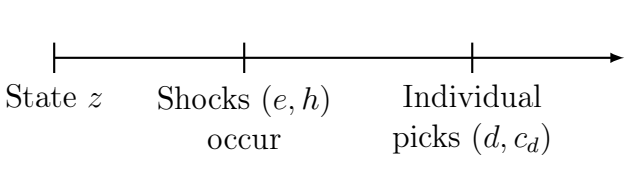
\includegraphics{figures/timeline_static.png}

\textbf{Shocks:}

\begin{itemize}
\tightlist
\item
  \(e = (e_0 , e_1) \in \mathbb{R}^2\) only discrete choice for one
  alternative, drawn from \(\epsilon\)
\item
  \(h \in \mathbb{R}\) shocks discrete and continuous for both
  alternatives, drawn from \(\eta\)
\end{itemize}

\textbf{State Variables:} \(z\)

\textbf{Choices:}

\begin{itemize}
\tightlist
\item
  \(d \in {0,1}\) discrete choice
\item
  \(c_d \in \mathbb{R}\) continuous choice given \(d\)
\end{itemize}

\textbf{Payoffs:}

\[\max_{d, c_d} V_d(c_d,z,h,e_d)\]

\subsection{Framework: Assumptions}\label{framework-assumptions}

\begin{enumerate}
\def\labelenumi{\arabic{enumi}.}
\tightlist
\item
  \textbf{Additive Separability:} \(e\) enters the payoff additively,
  for each \(d\) \[V_d(c_d,z,h,e_d) = \tilde{v}_d (c_d,z,h) + e_d\]
\end{enumerate}

Assumption 1 implies: conditional policy \(c^{*}_d\) does not depend on
\(e\)

\begin{enumerate}
\def\labelenumi{\arabic{enumi}.}
\setcounter{enumi}{1}
\tightlist
\item
  \textbf{Instrument:} \(z = (x,w)\) and \(w\) does not enter the
  conditional continuous choice
  \[\tilde{v}_d (c_d,z,h) = v_d (c_d,x,h) + m_d(x,w,h)\]
\end{enumerate}

Assumption 2 implies: conditional policy \(c^{*}_d\) does not depend on
\(w\)

\subsection{Framework: More
Assumptions}\label{framework-more-assumptions}

\begin{enumerate}
\def\labelenumi{\arabic{enumi}.}
\setcounter{enumi}{2}
\tightlist
\item
  \textbf{Monotonicity:} \(v_d\) is twice continuously differentiable
  and \(\frac{\partial^2v_d(c_d,z,h)}{\partial c_d \partial h} > 0\)
\end{enumerate}

Assumption 3 implies:

\begin{itemize}
\tightlist
\item
  given \(d\) and \(x\), \(c^{*}_d(z,h)\) is one-to-one with \(h\)\\
\item
  the framework requires non-trivial continuous choice for each discrete
  choice
\end{itemize}

\begin{enumerate}
\def\labelenumi{\arabic{enumi}.}
\setcounter{enumi}{3}
\item
  \textbf{Shocks:} Conditional on \(X = x\), (i) \(W, \eta, \epsilon\)
  are mutually independent, (ii) \(\eta\) drawn from \(Uniform(0,1)\),
  (iii) \(\epsilon\) is continuouslly distributed with full support/,
  and (iv) \(\max_{c} \tilde{v}_d (c, x,w,h) < \infty\) for all
  \((x,w,h,d)\).
\item
  \textbf{Instrument Relevance:} For every \(x\),
  \(P(D = 0 | \eta = h, X = x, W = 1) \neq P(D = 0 | \eta = h, X = x, W = 0)\),
  for all \(h \in \mathcal{H} \backslash \mathcal{K}_x\), where
  \(\mathcal{K}_x\) is a possibly empty finite set.
\end{enumerate}

\subsection{Framework: Example - Static Energy
Demand}\label{framework-example---static-energy-demand}

\textbf{Decision Problem}:
\[\max_{d, c_d} \{v_d(c_d,x,h) + m_d(x,w,h) + e_d \}\]

\textbf{Energy Sources}: Discrete \(d = 0 \text{ or } 1\)

\textbf{Energy Demand}: Continuous \(c_0\) and \(c_1\)

\textbf{Characteristics}: \(x\), cost, income, etc

\textbf{Instrument}: \(w\), e.g.~previous energy source

\textbf{Taste Shock}: \(e_d\) specific to sources

\textbf{Demand Shock}: \(h\), shifts \(c_d\) for
\(d = 0 \text{ and } 1\), also enters the discrete choice

\subsection{Framework: Example - Implication of
Assumptions}\label{framework-example---implication-of-assumptions}

\textbf{Decision Problem}:
\[\max_{d, c_d} \{v_d(c_d,x,h) + \underbrace{m_d(x,w,h) + e_d}_{\text{discrete choice shock}}\}\]

\textbf{Instrument Shifts Conditional Choice Probability:} \[
\begin{align}
 &P(D = 0 | \eta = h, X = x, W = 1) \\
 &= P(e_0 - e_1 > \max_{c_1}v_1(c_1,x,h) - \max_{c_0}v_0(c_0,x,h)+ \\
 & m_1(x,w,h)-m_0(x,w,h)| \eta = h, X = x, W = w)
\end{align}
\]

\subsection{Framework: Example - Implication of
Assumptions}\label{framework-example---implication-of-assumptions-1}

\textbf{Instrument Shifts Conditional Choice Probability:} \[
\begin{align}
 &P(D = 0 | \eta = h, X = x, W = 1) \\
 &= P(e_0 - e_1 > \max_{c_1}v_1(c_1,x,h) - \max_{c_0}v_0(c_0,x,h)+ \\
 & m_1(x,w,h)-m_0(x,w,h)| \eta = h, X = x, W = w)
\end{align}
\]

since \((e_0,e_1) \perp (W,\eta) | X = x\) (A4) and

\(\max_{c_1}v_1(c_1,x,h) - \max_{c_0}v_0(c_0,x,h)\) independent of \(w\)
(A2).

We have that (A5) is equivalent to an assumption on discrete choice
shock: \[
\begin{align}
 P(D = 0 | \eta = h, X = x, W = 1) \neq P(D = 0 | \eta = h, X = x, W = 0) \\
 \iff m_1(x,w=1,h)-m_0(x,w=1,h) \neq m_1(x,w=0,h)-m_0(x,w=0,h)
\end{align}
\]

\subsection{Identification: Static}\label{identification-static}

\textbf{Data:} \((D,C,W)\), we omit \(X\) as it is exogenous and
\(\epsilon,W,\eta\) mutually independent when fixing on \(X=x\)

\textbf{Structures to be Identified:}\\
-Conditional Continuous Choices: \(c^{*}_d(h)\)\\
-Conditional Choice Probability: \(P(D = d | \eta = h, W = w)\)\\
-Indirect Payoffs: \(\max_{c}v_d(c,h)\) and \(m_d(w,h)\)

\textbf{Reduced Forms Recovered from Data:}\\
-Distribution of Continuous Choice given \(d\) and \(w\):
\(F_{C_d|d,w}(c_d) = P(C_d < c_d | d, w)\)\\
-Choice Probability given \(w\): \(p_{D|w}(d) = P(d|w)\)

\subsection{Identification: Lemmas}\label{identification-lemmas}

\textbf{Lemma 1:} Under Assumption 3 and 4,
\(F_{C_d|d,w}(c_d) = P(C_d < c_d| d, w)\) is continuously differentiable
and strictly increasing, for \(d = 0,1\).

-\textbf{Intuition:} \textbf{Monotonicity} implies that \(h\) and
\(c^{*}_d(h)\) are one-to-one given \(d,w\). We have that
\(F_{\eta|d,w}\) is continuously differentiable and strictly increasing,
so \(F_{C_d|d,w}\) inherits these properties.

\textbf{Lemma 2:} Under Assumption 5,
\(\frac{\partial F_{C_d|d,1}(c_d)p_{D|1}(d)}{\partial c_d} \neq \frac{\partial F_{C_d|d,0}(c_d)p_{D|0}(d)}{\partial c_d}\)
for \(d = 0,1\), where \(h \in \mathcal{H} \backslash \mathcal{K}_x\),
where \(\mathcal{K}_x\) is a possibly empty finite set.

-\textbf{Intuition:} Given the same discrete choice, individual with
different \(w\) experienced different distributions of \(h\) shock.
Since \(h\) and \(c^{*}_d(h)\) are one-to-one, we can take this
restriction to data.

\subsection{Identification: Conditional Continuous
Choice}\label{identification-conditional-continuous-choice}

\textbf{Goal}: Identify \(c^{*}_0(h)\) and \(c^{*}_1(h)\)\\
\textbf{Challenge}:
\(P(\eta < h | D=d) = P(C_d < c^{*}_d(h)| D=d) \implies \\ c^{*}_d(h) = F_{C_d|d}^{-1}(P(\eta < h | D=d))\)
\(P(\eta < h | D=d)\) unobserved!

\textbf{Identification Intuition: Fixing an \(h\) and \(w=1\), we have}
\[
\begin{align}
 h &= P(\eta < h)\\
   &= P(\eta < h | W = 1) \hspace{1cm} [A4]\\
   &= P(\eta < h | D=0, W = 1)P(D=0| W = 1) + \\
   &P(\eta < h | D=1, W = 1)P(D=1| W = 1)\\
   &= P(C_0 < c^{*}_0(h) | D=0, W = 1)P(D=0| W = 1) + \\
   &P(C_1 < c^{*}_1(h) | D=1, W = 1)P(D=1| W = 1)\\
   &= F_{C_0|0,1}(c^{*}_0(h))p_{D|1}(0) + F_{C_1|1,1}(c^{*}_1(h))p_{D|1}(1)
\end{align}
\]

\subsection{Identification: Conditional Continuous
Choice}\label{identification-conditional-continuous-choice-1}

\textbf{Identification Intuition: Fixing an \(h\) and \(w=1\), we have}
\[
\begin{align}
 h = F_{C_0|0,1}(c^{*}_0(h))p_{D|1}(0) + F_{C_1|1,1}(c^{*}_1(h))p_{D|1}(1)
\end{align}
\] Note that \(F_{C_d|d,w}(.)\) and \(p_{D|w}(.)\) are observed from
reduced form. We have two unknowns: \(c^{*}_0(h)\) and \(c^{*}_1(h)\),
but also an extra equation from \(w=0\). Thus we can solve for the CCCs
for each \(h\).

\textbf{Theorem 1} For every reduced form compatible with the structural
model, there exist unique conditional continuous choice (CCC) functions
\(c_d(h)\), \(d=1,0\) that are strictly increasing and satisfy:

\[
\begin{align}
 h = F_{C_0|0,w}(c_0(h))p_{D|w}(0) + F_{C_1|1,w}(c_1(h))p_{D|w}(1) \hspace{1cm} \text{for $h \in [0,1]$, $w = 0,1$}
\end{align}
\] Intuition as above, proof establishes uniqueness.

\subsection{Identification: Conditional Choice Probability and
Payoffs}\label{identification-conditional-choice-probability-and-payoffs}

\textbf{CCP}: Identify \(P(D = d | \eta = h, W = w)\)

\textbf{Challenge}: \(\eta\) unobserved

\textbf{Solution}: Given \(c^{*}_0(h)\) and \(c^{*}_1(h)\) are
identified and strictly monotonic, we can recover
\(\eta = (c^{*}_D(h))^{-1}(C)\) from data \((D,C)\). It is then as if
\((D,C,W,\eta)\) are all observed.

\textbf{Payoffs}: Identified, but depend on how the CCCs and CCPs relate
to the utility/value function.

\subsection{Framework: Dynamic}\label{framework-dynamic}

\textbf{Assumptions D1-D3}: Assumptions on the curent utility, similar
to the static version but with \(t\) subscript.

\begin{enumerate}
\def\labelenumi{\arabic{enumi}.}
\setcounter{enumi}{5}
\tightlist
\item
  \textbf{Conditional Independence}: For all \(x_t \in X\),
  \(w_t \in W\), \(e_t \in \epsilon\), \(h_t \in H\), \[
  \begin{align}
    f_{X_{t+1},W_{t+1},\epsilon_{t+1},\eta_{t+1}|x_{t},w_{t},c_{t},d_{t},e_{t},h_{t}}(x_{t+1},w_{t+1},e_{t+1},h_{t+1}) = \\
    f_{X_{t+1},W_{t+1}|x_{t},w_{t},c_{t},d_{t}}(x_{t+1},w_{t+1})f_{\epsilon}(e_{t+1})f_{\eta}(h_{t+1})
  \end{align}
  \]
\item
  \textbf{Instrument Transition Exclusion}: For all \(x_t \in X\),
  \(w_t \in W\), the current instrument is excluded from the transition
  density: \[
  \begin{align}
    f_{X_{t+1},W_{t+1}|x_{t},w_{t},c_{t},d_{t}}(x_{t+1},w_{t+1}) =
    f_{X_{t+1},W_{t+1}|x_{t},c_{t},d_{t}}(x_{t+1},w_{t+1})
  \end{align}
  \] Assumption 6 and 7 are required to fit the dynamic problem into the
  general framework we developed before.
\end{enumerate}

\subsection{Framework: Dynamic}\label{framework-dynamic-1}

\textbf{The Dynamic Decision Problem:}
\[V_t(z_t) := \mathbb{E}[\sum_{\tau=t}^{T} \max_{D,C_{D \tau}} u_{D\tau}(C_{\tau}, X_{\tau}, \eta_{\tau}) + m_{D \tau}(X_{\tau}, W_{\tau}, \eta_{\tau}) + \epsilon_{D \tau}] \]

We can write it recursively, using assumption 6 and 7 \[
\begin{align}
V_t(z_t) := \mathbb{E}_{\epsilon,\eta}[&\max_{D,C_{D \tau}}[ u_{dt}(c_{dt}, x_{t}, \eta_{t}) + m_{dt}(x_{t}, w_{t}, \eta_{t}) + \epsilon_{dt} + \\
& \beta \mathbb{E}_{Z_{t+1}}[V_{t+1}(Z_{t+1})|X_t=x_t,C_t=c_{dt},D_t=d_t]]] 
\end{align}
\] With the instrument excluded from the state transition, the
continuation value term does not depend on \(w\).

\subsection{Framework: Dynamic}\label{framework-dynamic-2}

Define the conditional value function:
\[v_{dt}(c_{dt},x_t,\eta_t) = u_{dt}(c_{dt}, x_{t}, \eta_{t}) + \beta \mathbb{E}_{Z_{t+1}}[V_{t+1}(Z_{t+1})|X_t=x_t,C_t=c_{dt},D_t=d_t]\]

Reformulate the per-period problem, we have:
\[\max_{d_t, c_{dt}} \{v_{dt}(c_{dt},x_t,h_t) + m_{dt}(x_t,w_t,h_t) + e_{dt} \}\]
which is of the same form as our static problem.

\textbf{Lemma 3:} Under Assumptions D1-D3, 6, and 7, Assumption 1, 2, 3
are satisfied for the conditional value function in the dynamic setup.

-\textbf{Intuition:} Assumption 1 (AS) follows from D1.\\
Assumption 2 (Instrument) follows from D2 + 7 (Instrument Transition
Exclusion).\\
Assumption 3 (Monotonicity) follows from D3 + 6 (CI).\\

\(\frac{\partial^2v_{dt}(c_{dt},x_t,h_t)}{\partial c_{dt} \partial h_t} = \underbrace{\frac{\partial^2u_{dt}(c_{dt},x_t,h_t)}{\partial c_{dt} \partial h_t}}_{>0 \text{, by } D3} + \underbrace{\frac{\partial^2 \mathbb{E}_{Z_{t+1}}[V_{t+1}(Z_{t+1})|X_t=x_t,C_t=c_{dt},D_t=d_t]}{\partial c_{dt} \partial h_t}}_{=0 \text{, by } CI} > 0\)

\subsection{Framework: Dynamic Example}\label{framework-dynamic-example}

We still need an instrument, the author proposes the previous discrete
choice \(W_t = D_{t-1}\).

\textbf{Decision Problem}:
\[\max_{d_t, c_{dt}} \{v_{dt}(c_{dt},x_t,h_t) + m_{dt}(x_t,w_t,h_t) + e_{dt} \}\]

\textbf{Energy Sources}: Discrete \(d_t = 0 \text{ or } 1\)

\textbf{Energy Demand}: Continuous \(c_{0t}\) and \(c_{1t}\)

\textbf{Characteristics}: \(x\), cost, income, etc

\textbf{Instrument}: \(w\), e.g.~previous energy source

\textbf{Taste Shock}: \(e_{dt}\) specific to sources

\textbf{Demand Shock}: \(h_t\), shifts \(c_{dt}\) for
\(d = 0 \text{ and } 1\), also enters the discrete choice

\subsection{Framework: Dynamic
Example}\label{framework-dynamic-example-1}

The author argues:

\begin{enumerate}
\def\labelenumi{\arabic{enumi})}
\item
  conditional on current source of energy \(d_t\) and \(x_t\), future
  \(w_{t+1}\) is known and \(x_{t+1}\) is unlikely to be influenced by
  past choice {[}defending Assumption 7, Transition Exclusion{]}
\item
  conditional on current source of energy \(d_t\) and \(x_t\), past
  choice unlikely to enter current utility function {[}defending
  Assumption D2, Exclusion{]}
\item
  past choice likely relevant if there is a switching cost {[}defending
  Assumption 5, Relevance{]}
\end{enumerate}

\subsection{Identification: Dynamic}\label{identification-dynamic}

As before, we are interested in identifying the CCCs \(c^{*}_{dt}\)\\
CCPs \(P(D_t = d_t | \eta_{t} = h_{t}, X_t = x_t, W_t = w_t)\), the
transition laws, and the value function parameters.

\textbf{Data:} \((D_t,C_t,X_t,W_t,t)\)

\textbf{Reduced Forms:}
\(R = \{P(D=d_t|X_t=x_t,W_t=w_{t}), F_{C_{dt}|d_t,x_t,w_t}(.)\}\)

For CCCs and CCPs, we proceed as before, exploiting our instrumental
variable.

For transition laws are non-parametrically identified from data.

The value functions are identified by extra assumptions on the
\(\epsilon_t\) term and on the current utility function, using existing
results.

\subsection{More in the paper}\label{more-in-the-paper}

-With unobserved types

-Two-step Estimation




\end{document}
